\documentclass[a4paper, 11pt]{article}

\usepackage{geometry}
\geometry{a4paper,left=30mm,right=30mm, top=35mm, bottom=30mm}

\usepackage[english]{babel}
\usepackage[utf8]{inputenc} 
\usepackage[T1]{fontenc}
\usepackage{amsmath}
\usepackage{amssymb}
\usepackage{fancyhdr}
\usepackage{graphicx}
\usepackage{hyperref}
\usepackage{csquotes}

\usepackage{lastpage} % Seitenzahlen

\pagestyle{fancy}
\usepackage{amsmath}
\usepackage{tabularx} %schöne tabellen
\parindent0pt %einrücken verhindern
\renewcommand{\familydefault}{\sfdefault} % use sans fonts


\cfoot{\thepage  \ / \pageref{LastPage}}

\usepackage[
backend=biber,
%style=ieee,
citestyle=authoryear
]{biblatex}

\graphicspath{{./images/}}

% % % % % % % % % % % % % % % % % % % % % % % %
% % % % % % % % % % % % % % % % % % % % % % % %
\newcommand{\thesis}{Bachelor Thesis}
\newcommand{\topic}{Using Approximate Bayesian Computation to Infer the Number of Populations from SNP Genotype Data}
\newcommand{\modul}{Bachelor Thesis}
\newcommand{\supervisor}{Supervisors: Manfred Opper, \\ Olivier Fran\c{c}ios, \\ Michael Blum}
 \newcommand{\name}{Fabian Bergmann}
\newcommand{\datum}{\today}
% % % % % % % % % % % % % % % % % % % % % % % %
% % % % % % % % % % % % % % % % % % % % % % % %


\addbibresource{sources.bib}

\begin{document} 

%%% Kopfzeile linker Bereich
%      gerade Seite   ungerade Seite
\lhead[ \leftmark   ]{\textbf{\modul}}
%%% Kopfzeile mittlerer Bereich
%      gerade Seite   ungerade Seite
\chead[\rightmark   ]{\rightmark{}}
%%% Kopfzeile linker Bereich
%      gerade Seite             ungerade Seite
\rhead[\textbf{text}]{\name}


	%-- Deckblatt --						      
  \title{\textbf{\thesis\\[0.5cm] \Large{\topic} \\[1.5cm]}
	\author{%\tutorium\\ \\
		Fabian Bergmann, 372918\\ \\ \\ \\ \\ \\ \\ \\ 
		Pages: \pageref{LastPage} \\ \\ \\ \\
		}
	\normalsize{\supervisor}} %Thema ändern	
	\date{Submission Date: \datum} %Datum ändern
	\maketitle
	\newpage
	
\renewcommand{\labelenumi}{\alph{enumi})}
\renewcommand{\labelenumii}{(\roman{enumii})}
\renewcommand{\labelenumiii}{\arabic{enumiii}.}
%\renewcommand{\labelenumii}{\textbf{-}}	
%-- Eigentlicher Text --

\section{Introduction}
In population genetics theoretical models are constructed according to devised hypotheses to investigate the population structure and its evolution for some organisams at interest. Usually for this purpose the validity of a certain model is evaluated by analysing the underlying genotype data of the organisms. Models are often susceptible to the realistic choice of hyperparameters, such that for example the likelihood of a model with a certain hyper parameter greater is than for a much more realistc hyper parameter. Since for many models the declaration of the number of populations in the given data is crucial to infer the remaining parameters, a successful and stable technique for determining this parameter would lead to a significant facilitation for the inference process. However, so far no automated solution exists that satisfyingly alleviate this concern. \\
Throughout the following pages an approximate bayesian computation method will be presented that intends to deliver a reasonable estimate for the number of populations in SNP genotype data. It is based on a generalisation of currently used approaches, that attempt to exploit the behaviour of the spectrum of a clustered data matrix. The eigenvalues will moreover also make up the utilised summary statistics. The likelihood function for this problem is elusive, therefore a gradient boosting tequnique with decision trees wil be employed to bypass its explicit computation. \\
Gradient Boosting is a supervised machine learning method, thus it requires a significant amount of data for training and testing. Real world genotype data however is too extensiv to acquire in such a magnitude as is necessary, therefore an artificial data set is simulated and used. The generation of the artificial data follows commonly accepted theories for the simulation of population structure.

\subsection{Problem}
Given the genotype data of individuals, organised in a matrix $X$ where each row corresponds to an individual, the task is to infer how many populations $K$ are present in $X$. A population is a "group of organisms of the same species living within a sufficiently restricted geographical area so that any member can potentially mate with any other member of the oppisite sex" \cite{hartl1997principles}. Especially due to genetic drift, the change of the allele frequencies in a population that occurs because of finite random sampling from the available gene pool, populations are destinguishable in their genetic information, although they might have split from a single population a reasonable amount of generations ago. For further information the reader is referred to \cite{hartl1997principles}. Therefore, if a sufficient amount of genetic information is used to span the feature space, usually in the form of genetic variations found at genetic markers, individuals should cluster together with other individuals of the same population as their genetic data is more homogenous \textbf{add more reasoning???, law of large numbers???}. The number of populations $K$ should accord with $K$ clusters found in the feature space, so the problem simplifies to identifying the number of clusters found in the data matrix $X$. \textbf{give a definition for clusters???, measure of genetic distance???}

\subsection{Approaches currently used}
A natural approach for problems involving clustering, would be to use a well established method and adapting it to infer the number of clusters, such as by maximising the likelihood of an expactation maximisation in combination with a model quality estimator like the Akaike Information Criterion to avoid overfitting. In general maximising the likelihood with regard to a theoretical model of the population structure is always a possible approach, however makes the estimation of the number of populations highly dependable on the a-priori assumptions of the model for what determines mathematically a new population. \cite{falush2003inference} Different assumptions from different models could lead to different estimations, which would undermine their comparability. Nevertheless, a maximum-likelihood approach was implemented in the software STRUCTURE \cite{pritchard2000inference} \cite{falush2003inference} and widely applied \cite{rosenberg2002genetic} \cite{harter2004origin} \cite{rosenberg2001empirical}. Furthermore, in some cases, especially for data that involves a high number of populations, a very distinctive maximum is not obtained, for the maximum-likelihood function tends to be smoother as higher values are examined \textbf{more explanation???}. Some approaches add further heuristics, such as also taking the second order rate of change of the likelihood function into consideration \cite{evanno2005detecting}, which however appears more like mending the performance of an approach that was solely conceived as preliminary remedy \cite{pritchard2000inference}.\\

A more "modern" approach involves the insight that a cluster structure is also resembled in a structured form in the spectrum of the respective data matrix. The connection between the spectrum and a matrix was first discovered in graph theory \cite{donath1973lower} \cite{fiedler1973algebraic} and later introduced into machine learning \cite{shi2000normalized} \cite{meila2001random} \cite{ng2002spectral}, for further information see \cite{von2007tutorial}.

\subsubsection{Key words}

\begin{itemize}
\item \textbf{Chromosome:} A DNA molecule that encodes genetic information.

\item \textbf{Gene:} A DNA (or RNA) sequence that specifies the structure of a particular functional molecule.

\item \textbf{Locus:} A particular position on the chromosome, like the position of a specific gene.

\item \textbf{Allele:} A variant form of a given gene. Different alleles can lead to distinct phenotypic traits.

\end{itemize}

\section{Modelling}

\subsection{Biological Background}
The subsequent admixture model, follows a model proposed by \cite{pritchard2000inference}. 

\textbf{model assumptions}

A population is defined by its allele probabilites, whereby the members of the population are approximately homogenous. The allele probalities are a categorical distributions over the possible alleles at each locus, so how often a genetic variant appears in a population. \textbf{mention linkage disequilibrium and hardy-weinberg equilibrium} So at principal, to simulate a new population, its allele probabilities have to be determined. The simulated data the modell produces is supposed to resemble SNP data, where no distinction is made between the different variants of a mutation, but solely if a mutation at ll exists compared to an undetermined hypothetical origin population. Furthermore, ploidity is also neglected, so it is assumed the genetic data is aploidic, since \textbf{ploidity adds nothing unique for the means of inference. citation needed} \\
The following modell has a hierarchical structure starting with allele probabilities that are derived from an unseen ancestral population. Let $p^{A}_{l}$ denote the probability, sampled from a uniform distribution, of an individual from the ancestral population $A$ having a variation at locus $l$. Subsequently, following the by \cite{falush2003inference} established F-model, for each population $k$ an F-value $F^{k}$ is sampled from a \textbf{add distribution}. These are used to derive the mutation probabilities of population $k$ at locus $l$:

\begin{align*}
p^{k}_l = beta(p^{A}_{l} \frac{1 - F^k}{F^k}, (1-p^{A}_{l}) \frac{1 - F^k}{F^k})
\end{align*}

The probability values are joined to a vector $p^k$ and then merged with all other $K$ populations to a matrix $\mathbf{F} = [p^1 p^2 \ldots p^K]^T$ of size $K \times L$, where $L$ is the number of locus, such that each column of $\mathbf{F}$ gives the probabilities of each population for a specific locus $l$. \\

\textbf{explain reasoning for F-values}

To introduce the prospect of mating between individuals from different populations, possibilities of simulating admixed individuals and even whole admixed populations are added according to the admixture model presented in \cite{pritchard2000inference}. An admixed individual is defined by possessing a mixture of genetic data from various populations. The mixture is a weighting modeled by a categorical distribution according to the influence of each population on the individual. For an individual $i$ the weights $q_i$ are sampled from a dirichlet distribution with $K$ influence paramaters $j_1, j_2, \ldots, j_K$ each corresponding to a population, thus $q_i \sim dir(j_1, j_2, \ldots, j_K)$. A non admixed individual $j$ also receives mixing parameters with the difference that the only non-zero value is a one at position $k$, indicating that the individual belongs to population $k$, so $q_j = [0_1, \ldots, 1_k, \ldots, 0_K]^T$. All $M$ individuals are combined to a mixing matrix $\mathbf{Q} = [q_1,q_2, \ldots q_M]^T$ of dimensions $M \times K$. \\

\textbf{add description of influencing parameters}

The mixing weights of each individual are subsequently applied over the mutation probabilites of all populations at each locus, which equals to the multiplication of both established matrices $\mathbf{P} = \mathbf{Q}\mathbf{F}$. The resulting matrix $\mathbf{P}$ of dimension $N \times L$ holds the mutation probabilities of each individual for each locus. By using each entry of $\mathbf{P}$ to sample a value from a bernoulli \textbf{why bernoulli???} distribution, the simulated SNP genotype data for each individual is obtained. \\

\textbf{add modell relevance to real life ???}

%\begin{align*}
%\mathbf{Q} = \begin{bmatrix}
%q_1^T \\
%q_2^T  \\
%\vdots  \\
%q_n^T
%\end{bmatrix}
%\end{align*}




\newpage

\section{Theory}

\subsection{ABC}

To infer the number of populations $K$ expressed in a given dataset $X$ the conditional probability $P(K | X)$ with respect to $K$ is maximized. Since the large dimensionalities of the used datasets pose substantial computational difficulties, the datasets are summarized  in an effective manner, such that the approximation $P(K|X) \approx P(K | sum(X))$ is sufficient for the intended inference. Bayes' theorem then yields

\begin{align*}
P(K | sum(X)) = \frac{P(sum(X) | K) P(K)}{P(sum(X))}
\end{align*}

The calculation of the likelihood $P(sum(X) | K)$ however is intractable because \textbf{???}
To circumvent this problem the likelihood is implicitly calculated by employing a supervised learning method to estimate the posterior, such as a neural network or boosting decision trees. These methods are trained by trying to link summary statistics of datasets to the corresponding values for the number of populations. The prior $P(K)$ 
can be implicitly adjusted by changing the proportions of $K$ in the training data. Gradient boosting with decision trees is chosen in this case, for it has demonstrated good results for various classification problems citation needed. \textbf{??? Furthermore, some inuitive reasoning exists, as explained later on, for the use of decision trees in this particular case.}

\subsection{Choosing the Summary Statistics}

The choice of an adequate summary statistics is essentiell to obtain significant results. On the one hand a summary of the data is necessary to handle its large dimensionality, on the other hand the manner of summarisation has to be chosen carefully to sustain the vital information necessary for the inference, because each summarisation consequently forfeits some of the principal information. 

\begin{align*}
h(x) & = - \int_{-\infty}^{\infty} N(x|\mu, \Sigma)ln(N(x|\mu, \Sigma))dx \\
& = E[ln(N(x|\mu, \Sigma)] \\
& = E[ln(det(2\pi\Sigma)^{-\frac{1}{2}}e^{-\frac{1}{2}(x-\mu)^T\Sigma^{-1}(x-\mu)})] \\
& = \frac{1}{2} ln(det(2\pi\Sigma)) + \frac{1}{2} E[(x-\mu)^T \Sigma^{-1}(x-\mu)]\\
& = \frac{1}{2} ln(det(2\pi\Sigma)) + \frac{1}{2} E[trace(\Sigma^{-1}(x-\mu)^T (x-\mu))]\\
& = \frac{1}{2} ln(det(2\pi\Sigma)) + \frac{1}{2} E[trace(I)]\\
& = \frac{1}{2} ln(det(2\pi e \Sigma))
\end{align*}

The only non-constant factor influencing the entropy of a multivariate gaussian is the determinant of the respective correlation matrix.
Since any real symmetric matrix is diagonalisable, $det(\Sigma)$ breaks down to $det(\Sigma) = det(\mathbf{Q}^{-1}) \cdot det(\mathbf{\Lambda})\cdot det(\mathbf{Q}) = \prod_{i = 1} \lambda_{i}$, thus revealing that actually the eigenvalues of the correlation matrix are responsible for the magnitude of the entropy.
Furthermore, the multivariate Gaussian for a given mean and variance is the maximum entropy distribution, for a proof the reader is referred to \cite{cover2012elements}.

\textbf{Assume Data is linearly correlated??? connection of normal distribution to PCA}

\subsubsection{PCA - Introduction}

\textbf{introduction}
Principle component analysis is a statistical method that performs a basis transformation on a given data set, such that no linear correlations are anymore expressed by the data. Since the direction of a linear correlation corresponds to the direction of the highest variance in a concerning subspace, a new axis musst be aligned according that particular direction. \textbf{citation needed ???} This construction of the axes is done by requiering in an iterative manner each new axis to align with the direction that captures the most variance in the data, which however has not been captured by already established axes. \\
The differences between data points makes them destingiushable, but also determines the magnitude of the observed variance. Decreasing the variance in a data set by projecting it into a subspace, thus endagers destinguishability (in certain features or even in total), which is information. The amount of sustained variance after projecting the data into a subspace can, therefore act as an indicator for how much information was retained. So by always maximizing the captured variance of a newly added axis to the transformation, which is a subspace of the principal data set, the highest possible amount of information is retained for a projection into a subspace with a particular rank $K$ (under the assumption that variance corresponds to information). The subspace is spanned by the $K$ largest Eigenvectors \textbf{singular values ???} of the empirical covariance matrix, as is subsequently shown. \\
Let $S = \frac{1}{N}XX^T - \overline{X} \overline{X}^T$ denote the emperical covariance matrix of the data matrix $X$. Then the expression $u^TSu$ is the emprical variance of $u^TX$, which is the data $X$ projected on to the vector $u$.

\begin{align*}
u^T S u & = \frac{1}{N} u^T X X^T u - u^T \overline{X} \overline{X}^T u \\
& = \frac{1}{N} u^T X (u^T X)^T  -  \overline{u^TX} (\overline{u^TX})^T  \\
& = \frac{1}{N} (u^T X)^2 - (\overline{u^TX})^2
\end{align*}

The empirical variance is maximised with the restriction $\parallel x \parallel = 1$ because $u$ is supposed to be part of a new standard basis. \textbf{mention orthogonality ???}. By using a lagrange multiplier to add this restriction, the equation $\max\limits_{u} u^T \Sigma u - \lambda(u^T u - 1)$ is obtained.

\begin{align*}
 \frac{d}{du} (u^T \Sigma u - \lambda(u^T u - 1)) & = 0 \\
 \Sigma u - \lambda u & = 0 \\
 \Sigma u & = \lambda u 
\end{align*}

The solution coincides with the definition of the Eigenvectors, where $\lambda$ is the eigenvalue of $u$. Since $u$ should be maximised, the overall solution is the eigenvector belonging to the largest eigenvalue.

\subsubsection{In context to clustering}
Cluster analysis intends to group similar data points together. \textbf{what are the clustering assumptions??? distribution? group criteria? bounderies?}
Many connections between PCA and cluster analysis have been established \textbf{cite and give examples}.

Data that exhibits reasonable clustering possess a considerably unique structure. This structure also reveals itself to some degree in the orientation of the eigenvectors and the magnitude of the corresponding eigenvalues, such that they can be utilised to infer certain properties of the data, like the number of clusters as is the current intention. \\
Intuitively, for inferring the number of clusters, it is assumable \textbf{cluster assumptions} in a reasonable setting, including for example that each cluster has a similar amount of members, that the in-between variance between two distinct clusters is significantly greater than the variance whith-in a particular cluster. The in-between variance constitutes itself through the variance of the with-in variance of both concerning clusters and the distance between the clusters (under the assumption that outliers are possible, so cluster membership is not compulsive). While the with-in variance of a cluster is solely confined to the space assigned to that cluster, which concludes to a significantly smaller variance, espacially considering that the distance from the mean of each data point has a squared impact on the variance (definition of variance). \textbf{ Moreover, the with-in variance of a cluster is always the same (for $n \rightarrow \infty$) regardless of the vector it is projected on (is this true??? proof necessary - RMT), so each cluster can be summarised to its centroid}. For these reasons a new principal component will orient itself in such a way, that it effectively captures the remaining in-between variance of the clusters. \\
For $K$ many different population clusters $K-1$ significant PCs are obtained, thus allowing an inference of the number of populations. Considering only two clusters, a single significant PC would be observed that is oriented along a line connecting the two centroids of each cluster, as this would maximise the distance of the clusters after a projection on the PC and therefore maximise the variance after projection. In a general setting with $K$ clusters, the PCs would arrange themselves as linear combinations of the in-between variances, as the overall variance is maximised so all in-betwenn variances are taken into account. Since every cluster participates in $K-1$ in-between variances and capturing these in-between variances corresponds to determining the \textbf{exact??? (the centroids???} relative positions of the other cluster, a linear combination of exactly $K-1$ vectors are needed to locate the relative positions of the other clusters \textbf{proof necessary??? less: would mean a cluster is admixed, admixture = linear combination of existing clusters $\rightarrow$ contradiction | more: some in-between variance was not captured - contradiction to maximising variance, sufficient???}. \textbf{The centroids lie in the span of the first $K-1$ PCs ???}


\begin{figure}[h]
\caption{Projection of three populations and one admixed on to the firs two PCs and corresponding eigenvalues}
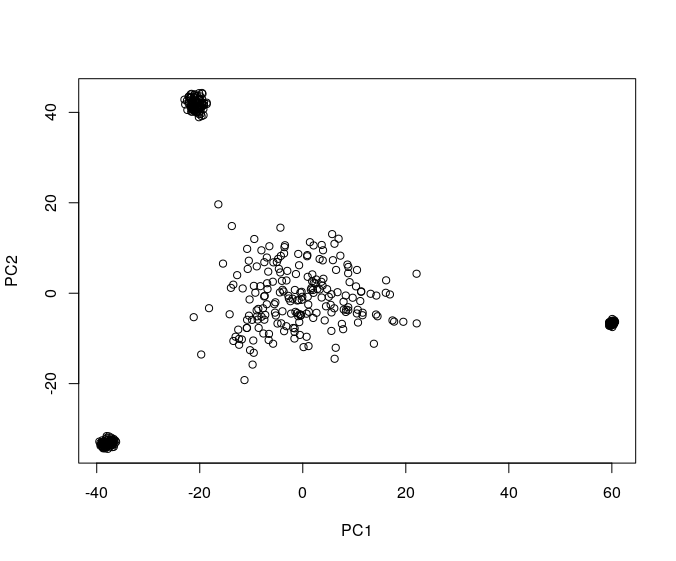
\includegraphics[scale=0.5]{Rplot_projection}
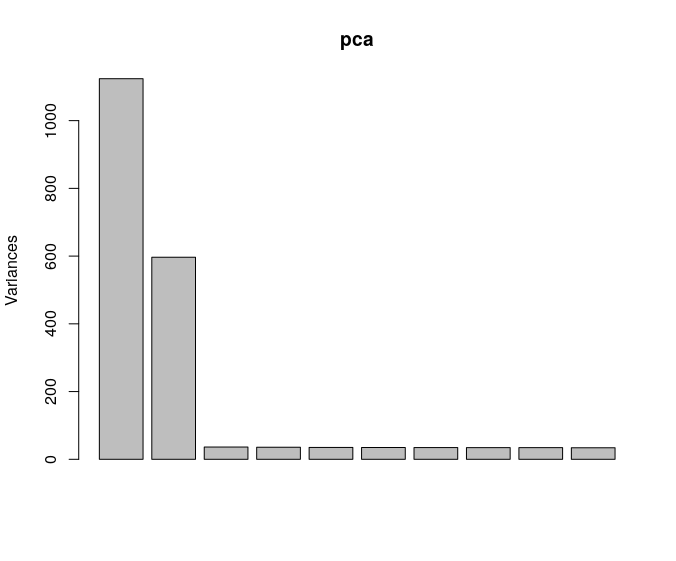
\includegraphics[scale=0.5]{Rplot_eigenvalues}
\\Three populations with F-values  of $0.1, 0.5, 0.9$ and $100$ individuals each were sampled. The admixed population derived the proportional weightings for its allele probabilites by sampling for each allele from a $Dir(8, 8, 8)$ distribution. $200$ individuals were sampled for the admixed. For this simulation $10000$ loci were simulated.
\centering
\end{figure}

The past mentions of population clusters solely referred to clusters that are not admixed. The introduction of admixed population clusters, however does not alter the previously established theory under certain assumptions. Admixed clusters are sampled from allele probability values that are subject to a weighting of the allele probability values of the non-admixed populations according to their involvement in the admixture \textbf{refer back to modell}. This is simply a linear combination, restricted to the coefficients being proportions, of the centroids of the other populations, hence it is situated in between non-admixed populations, meaning the centroid of an admixed population lies also in the span of the PCs spanning the non-admixed populations. \textbf{In general, the centroids of the non-admixed populations constitute the corners of a simplex, that determines if a population cluster is admixed - proof ???}. If a cluster lies within the simplex it is admixed (No cluster can lie outside the simplex). Since admixed clusters lie in between the non-admixed clusters, their influence concerning the maximisation of the variance is neglegible \textbf{further explanation needed???}.


\begin{figure}[h!]
\caption{Projection of three populations and one admixed on to the firs two PCs}
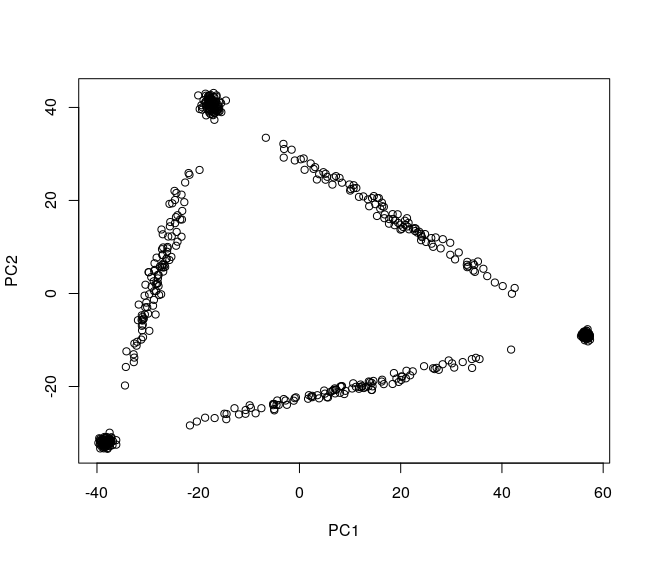
\includegraphics[scale=0.5]{Rplot_admixed_simplex}
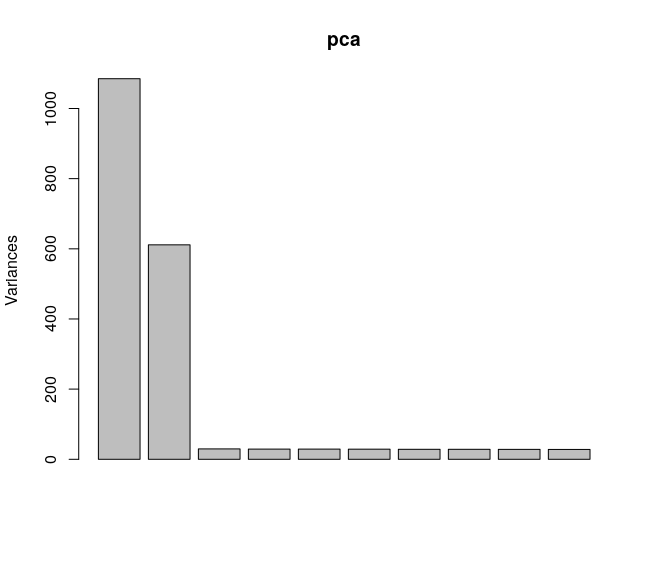
\includegraphics[scale=0.5]{Rplot_eigenvalues_simplex}
Three populations with F-values  of $0.1, 0.5, 0.9$ and $100$ individuals each were sampled. Between each pair of population clusters lies an admixed population sampled from a dirichlet with $5$s and a $0$ for not involved populations, which corresponds to a $beta(5, 5)$. Each admixed cluster holds $200$ individuals. The simulation used again $10000$ loci.

\centering
\end{figure}


\subsection{Difficulties}


\begin{figure}[h!]
\caption{Example of a difficult case}
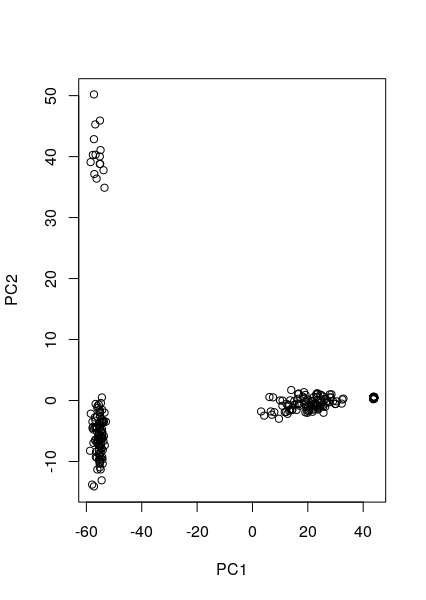
\includegraphics[scale=0.5]{Rplot_hard_example}
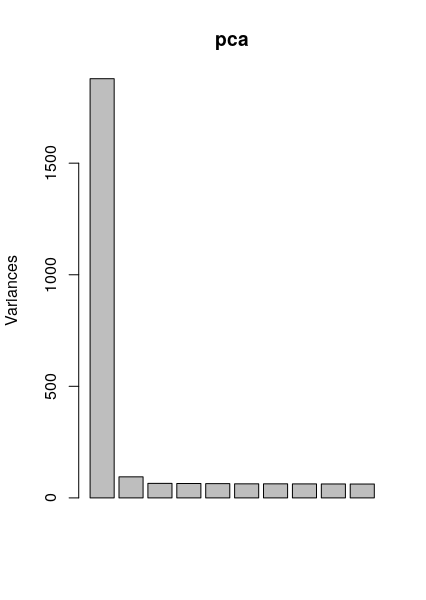
\includegraphics[scale=0.5]{hard_example_eigenvalues}
\\Three populations with F-values  of $0.05, 0.01, 0.99$. The first population with the smallest F-value has $15$ members, while the others have a $100$ each. The mixture proportions of the admixed population were sampled from a $Dir(0, 10, 30)$. $10000$ loci were simulated.

\centering
\end{figure}


\newpage

\subsection{RMT}

Let $\mathbf{A} = \frac{1}{n}\mathbf{X}\mathbf{X}^{T}$ be the empirical covariance matrix of $\mathbf{X}$ with $\mathbf{X}$ being an $m \times n$ matrix. $\lambda_{1},\lambda_{2}, \dots, \lambda_{m}$ are the corresponding eigenvalues of $\mathbf{A}$. The empirical spectral distribution (\textbf{ESD}) for  $\mathbf{M}$ is then given by:

\begin{align*}
F^{M}(x) = \frac{1}{m} \mid \{\lambda_{i} \leq x \mid i \leq m\} \mid
\end{align*}

Whereby $\mid \cdot \mid$ denotes the size of a set.
\\
\\
By assuming a theoretical setting in which $m, n \rightarrow \infty$ while $y = \frac{m}{n} \rightarrow (0, \infty)$ the Marchenko-Pastur Law extends the ESD to the continuous case.

Under the assumption that the entries of $\mathbf{X}$ are random variables iid distributed with mean $0$, it states that the probability density of the eigenvalues is given by:

\begin{align*}
p^{M}(x) = \frac{1}{2\pi xy \sigma^{2}}  \sqrt[]{(\rho_{+} - x)(x - \rho_{-})}
\end{align*}

where $\rho_{\pm} = \sigma^{2}(1 \pm \sqrt[]{y})^{2}$ and $\sigma^2$ is the variance of the random variables.
\\
\textbf{Insert Plot of distribution}
\\

\newpage

\section{Gradient Boosting}

\section{Results}

\section{Discussion}

\printbibliography

\end{document}
